\documentclass[11pt]{charter}

% El títulos de la memoria, se usa en la carátula y se puede usar el cualquier lugar del documento con el comando \ttitle
\titulo{Robot móvil de inspección y desinfección} 

% Nombre del posgrado, se usa en la carátula y se puede usar el cualquier lugar del documento con el comando \degreename
\posgrado{Carrera de Especialización en Sistemas Embebidos} 
%\posgrado{Carrera de Especialización en Internet de las Cosas} 
%\posgrado{Carrera de Especialización en Intelegencia Artificial}
%\posgrado{Maestría en Sistemas Embebidos} 
%\posgrado{Maestría en Internet de las cosas}

% Tu nombre, se puede usar el cualquier lugar del documento con el comando \authorname
\autor{Sergio Alberino} 

% El nombre del director y co-director, se puede usar el cualquier lugar del documento con el comando \supname y \cosupname y \pertesupname y \pertecosupname
\director{Claudio Verrastro}
\pertenenciaDirector{CNEA, UTN.BA} 
% FIXME:NO IMPLEMENTADO EL CODIRECTOR ni su pertenencia
\codirector{} % si queda vacio no se deberíá incluir 
\pertenenciaCoDirector{}

% Nombre del cliente, quien va a aprobar los resultados del proyecto, se puede usar con el comando \clientename y \empclientename
\cliente{Grupo de Inteligencia Artificial y Robótica}
\empresaCliente{Universidad Tecnológica Nacional - Facultad Regional Buenos Aires}

% Nombre y pertenencia de los jurados, se pueden usar el cualquier lugar del documento con el comando \jurunoname, \jurdosname y \jurtresname y \perteunoname, \pertedosname y \pertetresname.
\juradoUno{Nombre y Apellido (1)}
\pertenenciaJurUno{pertenencia (1)} 
\juradoDos{Nombre y Apellido (2)}
\pertenenciaJurDos{pertenencia (2)}
\juradoTres{Nombre y Apellido (3)}
\pertenenciaJurTres{pertenencia (3)}
 
\fechaINICIO{22 de junio de 2020}		%Fecha de inicio de la cursada de GdP \fechaInicioName
\fechaFINALPlanificacion{22 de Agosto de 2020} 	%Fecha de final de cursada de GdP
\fechaFINALTrabajo{22 de diciembre de 2020}		%Fecha de defensa pública del trabajo final


\begin{document}

\maketitle
\thispagestyle{empty}
\pagebreak


\thispagestyle{empty}
{\setlength{\parskip}{0pt}
\tableofcontents{}
}
\pagebreak


\section{Registros de cambios}
\label{sec:registro}


\begin{table}[ht]
\label{tab:registro}
\centering

\begin{tabularx}{\linewidth}{@{}|c|X|c|@{}}
\hline
\rowcolor[HTML]{C0C0C0} 
Revisión & \multicolumn{1}{c|}{\cellcolor[HTML]{C0C0C0}Detalles de los cambios realizados} & Fecha      \\ \hline
1.0      & Creación del documento                                                          & 27/06/2020 \\ \hline
1.1      & Cambios a partir de corrección del docente                                                                                																						   & 16/07/2020 \\ \hline
\end{tabularx}
\end{table}

\pagebreak



\section{Acta de constitución del Proyecto}
\label{sec:acta}

\begin{flushright}
Buenos Aires, \fechaInicioName
\end{flushright}

\vspace{2cm}

Por medio de la presente se acuerda con el Ing. \authorname\hspace{1px} que su Trabajo Final de la \degreename\hspace{1px} se titulará ``\ttitle'', consistirá esencialmente en el prototipo preliminar de un robot móvil útil para tareas semiautónomas de inspección y desinfección, y tendrá un presupuesto preliminar estimado de 600 hs de trabajo y \$20.000, con fecha de inicio \fechaInicioName\hspace{1px} y fecha de presentación pública \fechaFinalName.

Se adjunta a esta acta la planificación inicial.

\vfill

% Esta parte se construye sola con la información que hayan cargado en el preámbulo del documento y no debe modificarla
\begin{table}[ht]
\centering
\begin{tabular}{ccc}
\begin{tabular}[c]{@{}c@{}}Ariel Lutenberg \\ Director posgrado FIUBA\end{tabular} &  & \begin{tabular}[c]{@{}c@{}}Juan Carlos Gómz por \clientename \\ \empclientename \end{tabular} \vspace{2.5cm} \\ 
\multicolumn{3}{c}{\begin{tabular}[c]{@{}c@{}} \supname \\ Director del Trabajo Final\end{tabular}} \vspace{2.5cm} \\
\begin{tabular}[c]{@{}c@{}}\jurunoname \\ Jurado del Trabajo Final\end{tabular}     &  & \begin{tabular}[c]{@{}c@{}}\jurdosname\\ Jurado del Trabajo Final\end{tabular}  \vspace{2.5cm}  \\
\multicolumn{3}{c}{\begin{tabular}[c]{@{}c@{}} \jurtresname\\ Jurado del Trabajo Final\end{tabular}} \vspace{.5cm}                                                                     
\end{tabular}
\end{table}




\section{Descripción técnica-conceptual del Proyecto a realizar}
\label{sec:descripcion}

\begin{consigna}{black}
 La idea consiste en el desarrollo de una plataforma móvil que pueda ser controlada a distancia para inspeccionar zonas de difícil acceso o para proveer servicios de desinfección por efecto de rayos ultravioletas. Esto sería principalmente útil en instituciones médicas en las que es posible el contagio de enfermedades por la propagación de bacterias y virus en ambientes comunes.
La plataforma debería contar con una placa de procesamiento central (Edu-CIAA) que recibe datos directos (o pre-procesados por otra/s placa/s) y una placa de control para el accionamiento de motores y/o dispositivos adicionales (como puede ser el encendido de un tubo UV).
Adicionalmente, el robot podría llevar una cámara inalámbrica para dar mayor información sobre las zonas inspeccionadas. En la Figura \ref{fig:diagBloques} se presenta el diagrama en bloques del sistema. 

\vspace{25px}

\begin{figure}[htpb]
\centering 
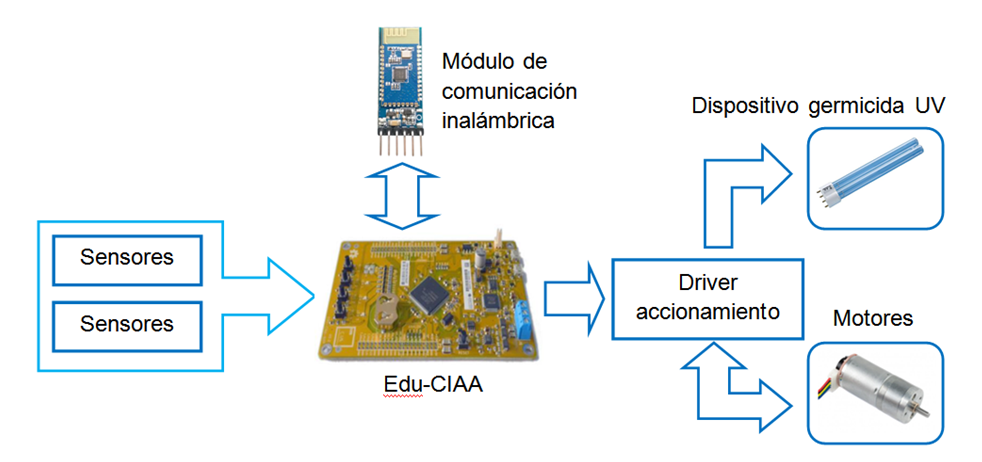
\includegraphics[width=.9\textwidth]{./Figuras/diagBloques.png}
\caption{Diagrama en bloques del sistema}
\label{fig:diagBloques}
\end{figure}

\vspace{25px}

Si bien existen plataformas robots similares, las mismas suelen estar fabricadas fuera del país, con lo que el costo de adquisición y transporte resultan particularmente elevados. Además, un desarrollo local documentado contaría con la posibilidad de soporte técnico dentro de las mismas instituciones involucradas.
La “Desinfección sin residuos químicos“ por luz ultravioleta ha demostrado efectividad como germicida, resultando letal para virus, bacterias, esporas de hongos y microorganismos superiores, ya que altera su ADN, evitando su reproducción.
Se prevé algún tipo de conectividad inalámbrica para control y obtención de datos, desde un dispositivo móvil. La idea es dejar preparada la plataforma para la posibilidad posterior de incorporación de módulos que provean servicios de valor agregado, como sensores específicos, posicionamiento GPS, etc.
La plataforma robot debe poder operar con baterías recargables que le den una autonomía aceptable para la tarea a realizar.
La presente propuesta espera ser aprovechada en el Grupo de Inteligencia Artificial y Robótica de la UTN - Facultad Regional Buenos Aires, El hardware resultante podrá ser utilizado también para la evaluación de algoritmos de Inteligencia Artificial, para aplicaciones en la industria local, y para actividades de docencia e investigación.

\end{consigna}


\section{Identificación y análisis de los interesados}
\label{sec:interesados}

\begin{consigna}{red} 

\begin{table}[ht]
%\caption{Identificación de los interesados}
%\label{tab:interesados}
\begin{tabularx}{\linewidth}{@{}|l|X|X|l|@{}}
\hline
\rowcolor[HTML]{C0C0C0} 
Rol           & Nombre y Apellido & Organización 	& Puesto 	\\ \hline
Auspiciante   &                   &              	&        	\\ \hline
Cliente       & \clientename      &\empclientename	&        	\\ \hline
Impulsor      & Secretaría de Ciencia, Tecnología e innovación productiva                  &\empclientename&        	\\ \hline
Responsable   & \authorname       & FIUBA        	& Alumno 	\\ \hline
Colaboradores &                   &              	&        	\\ \hline
Orientador    & \supname	      & \pertesupname 	& Director	Trabajo final \\ \hline
Usuario final & Personal de salud & Establecimientos hospitalarios 	&        	\\ \hline
\end{tabularx}
\end{table}


\end{consigna}



\section{1. Propósito del proyecto}
\label{sec:proposito}

\begin{consigna}{black}
El propósito de este proyecto es desarrollar un prototipo de plataforma móvil de observación para tareas semiautónomas de inspección y desinfección, con documentación completa para su reproducción a escala industrial. El dispositivo deberá poder controlarse a distancia para inspeccionar zonas de difícil acceso o para proveer servicios de desinfección por efecto de rayos ultravioletas. Esto sería principalmente útil en instituciones médicas en las que es posible el contagio de enfermedades por la propagación de bacterias y virus en ambientes comunes.
\end{consigna}

\section{2. Alcance del proyecto}\label{sec:alcance}
\begin{consigna}{black}
\vspace{-12mm}
\begin{itemize}
\item Diseño e implementación de una plataforma robot de dimensiones reducidas, con conectividad inalámbrica
\item Programación del firmware los módulos correspondientes. 
\item Programación del software de comunicaciones. 
\item Pruebas de funcionamiento.
\item Documentación del trabajo. 
\end{itemize}
El presente proyecto NO incluye: 
\begin{itemize}
\item La instalación y puesta en marcha del sistema completo de inspección y desinfección, en institución hospitalario (salvo que el tiempo disponible lo permita). 
\item El robot no monitoreará,  ni  realizará la carga de la batería.
\item No se incluye cargador.
\end{itemize}
\end{consigna}

\section{3. Supuestos del proyecto}
\label{sec:supuestos}

\begin{consigna}{black}
Para el desarrollo del presente proyecto se supone que: 

\begin{itemize}
\item Se contará con disponibilidad de los laboratorios e instrumental de la  Secretaría de Ciencia, Tecnología e innovación productiva. UTN. Buenos Aires, para cubrir la tarea de desarrollo.
\item Se dispondrá de tiempo durante la jornada laboral para la realización del mismo. 
\item  Se dispondrá de todos los componentes y herramientas necesarios. 
\end{itemize}

\end{consigna}

\section{4. Requerimientos}
\label{sec:requerimientos}
\begin{consigna}{black}
\vspace{-12mm}
\begin{enumerate}
\item Requerimientos funcionales
	\begin{enumerate}
	\item Capacidad de locomoción.  El robot debe ser capaz de desplazarse por medio de ruedas motorizadas, a través de superficies planas.
	\item Capacidad de percepción. El robot debe ser capaz de detectar y obtener información del medio. 
	\item Capacidad de comunicación inalámbrica.
	\item El robot deberá funcionar con alimentación a batería recargable.
	\item El proyecto debe ser extensible a una posible herramienta de enseñanza e investigación

	\end{enumerate}
\item Requerimientos no funcionales
	\begin{enumerate}
	\item El robot no debe resultar peligroso para el ambiente o las personas con las que podría interactuar.
	\item El diseño del robot debe respetar regulaciones en cuanto a radiación en el espectro ultravioleta.
	\item Se utilizarán componentes electrónicos disponibles comercialmente en Argentina.
	\end{enumerate}
\end{enumerate}
\end{consigna}

\section{Historias de usuarios (\textit{Product backlog})}
\label{sec:backlog}


\section{5. Entregables principales del proyecto}
\label{sec:entregables}
\vspace{-12mm}
\begin{consigna}{black}
\begin{itemize}
\item Prototipo funcional
\item Manual de uso
\item Diagrama esquemático del hardware
\item Códigos fuentes software
\item Informe final

\end{itemize}
\end{consigna}
\pagebreak


\section{6. Desglose del trabajo en tareas}
\label{sec:wbs}
\begin{consigna}{black}
\vspace{-12mm}
\begin{enumerate}
\item Planificación(50hs) 
	\begin{enumerate}
	\item Relevamiento de necesidades(10hs) 
	\item Análisis de requerimientos(20hs) 
	\item Confección de la planificación del proyecto(20hs) 
	\end{enumerate}
\item Diseño e implementación(155hs) 
	\begin{enumerate}
	\item Selección de materiales y componentes (10hs)
	\item Diseño de esquemáticos (35hs) 
	\item Construcción de hardware de control (35hs)
	\item Construcción de hardware de sensores (30hs)
	\item Integración de hardware (20hs)
	\item Pruebas funcionales (25hs) 
	\end{enumerate}
	\item Programación de Firmware (130hs) 
	\begin{enumerate}
	\item Programación software de control de motores  (20hs)
	\item Implementación de drivers para adquisición de datos de los sensores (20hs)
	\item Pruebas de funcionamiento (15hs)
	\item Programación de firmware de control reactivo para funcionamiento del robot (40hs) 
	\item Programación software de control comunicación(35hs) 
	\item Modificaciones para integración al software(10hs) 
	\end{enumerate}
	\item Construcción del prototipo (105hs) 
	\begin{enumerate}
	\item Diseño mecánico de la plataforma (20hs)
	\item Armado del prototipo(40hs)
	\item Pruebas funcionales de integración mecánica-electrónica (25hs)
	\item Ajuste de parámetros de funcionamiento (20hs)
	\end{enumerate}
	\item Programación de software de aplicación (85hs) 
	\begin{enumerate}
	\item Diseño de la interfaz de control (20hs) 
	\item Programación de la interfaz de control (40hs)
	\item  Pruebas y ajuste de la interfaz de control (25hs)
	\end{enumerate}
	\item Documentación y presentación (95hs) 
	\begin{enumerate}
	\item Informe de avances (10hs)
	\item Documentación del trabajo realizado (15hs) 
	\item Creación de manuales de uso (15hs) 
	\item Realización de Informe del proyecto (35hs) 
	\item Presentación final (20hs)
	\end{enumerate}
\end{enumerate}

Cantidad total de horas: (630 hs)

\end{consigna}
\pagebreak

\section{7. Diagrama de Activity On Node}
\label{sec:AoN}

\begin{consigna}{red}

\begin{figure}[htpb]
\centering 
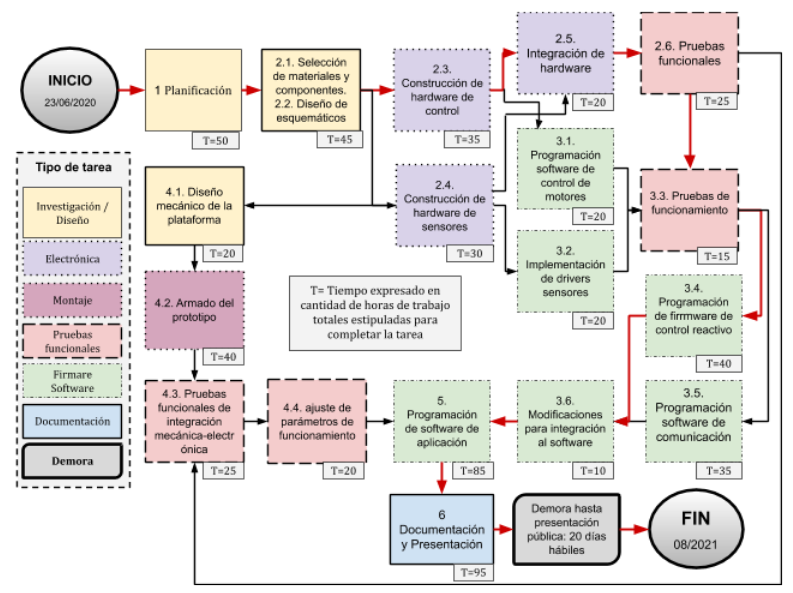
\includegraphics[width=.8\textwidth]{./Figuras/AoN.png}
\caption{Diagrama en \textit{Activity on Node}}
\label{fig:AoN}
\end{figure}

\end{consigna}
\pagebreak

\section{8. Diagrama de Gantt}
\label{sec:gantt}

\begin{consigna}{black}

\begin{figure}[htpb]
\centering 
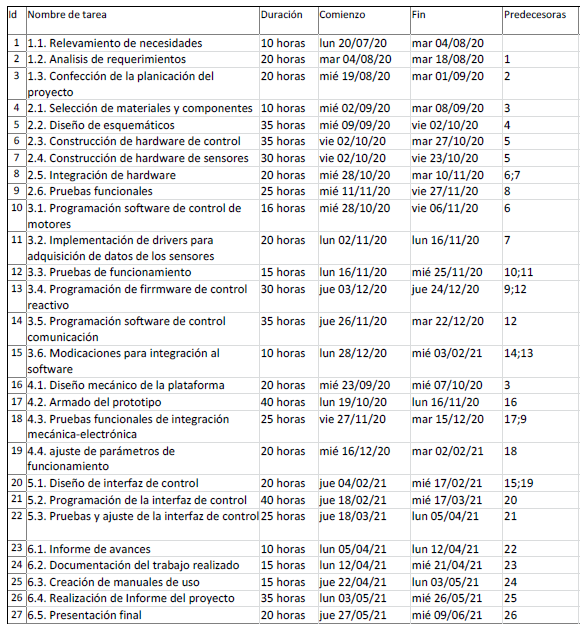
\includegraphics[width=\textwidth]{./Figuras/gantttabla.PNG}
\caption{Tabla de tareas de Gantt}
\label{fig:gantt}
\end{figure}

\begin{figure}[htpb]
\centering 
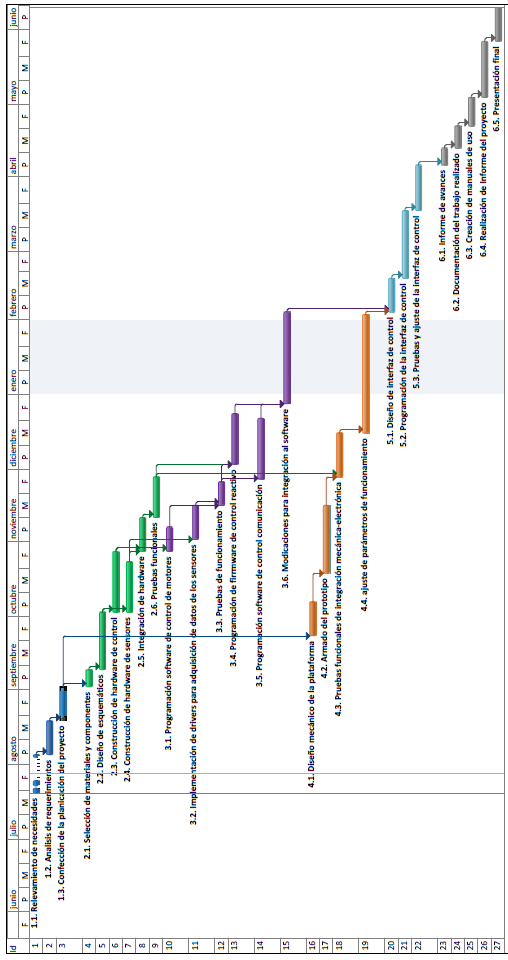
\includegraphics[width=.8\textwidth]{./Figuras/Gantt.PNG}
\caption{Diagrama de Gantt}
\label{fig:gantt}
\end{figure}
\end{consigna}
\pagebreak

\section{9. Matriz de uso de recursos de materiales}
\label{sec:recursos}

\begin{table}[htpb]
\label{tab:recursos}
\centering
%\resizebox{.9\textwidth}{!}{
\begin{tabularx}{\textwidth}{@{}|c|p{12em}|p{5em}|p{4.5em}|p{4.5em}|X|@{}}
\hline
\cellcolor[HTML]{C0C0C0} & \cellcolor[HTML]{C0C0C0} & \multicolumn{4}{c|}{\cellcolor[HTML]{C0C0C0}Recursos requeridos (horas)} \\ \cline{3-6} 
\multirow{-2}{*}{\cellcolor[HTML]{C0C0C0}\begin{tabular}[c]{@{}c@{}}Código\\ WBS\end{tabular}} 
& 
\multirow{-2}{*}{\cellcolor[HTML]{C0C0C0}\begin{tabular}[]{@{}c@{}}Nombre\\tarea\end{tabular}}
\centering
&  
PC con acceso a Internet & Placa de desarrollo & Taller de electrónica & Equipamiento mecánico / 3D \\ \hline
1 & Planificación & \multicolumn{1}{c|}{50hs}  &  &  &  \\ \hline
2.1 & Selección de materiales & \multicolumn{1}{c|}{10hs}  &  &  &  \\ \hline
2.2 & Diseño de esquemáticos & \multicolumn{1}{c|}{35hs}  &  &  &  \\ \hline
2.3 & Construcción de hardware de control & & & \multicolumn{1}{c|}{35hs} &    \\ \hline
2.4 & Construcción de hardware de sensores & & & \multicolumn{1}{c|}{30hs} &   \\ \hline
2.5 & Integración de hardware  &  &  & \multicolumn{1}{c|}{20hs} &  \\ \hline
2.6  & Pruebas funcionales    &  &  & \multicolumn{1}{c|}{25hs} &  \\ \hline
3.1 & Programación software de control de motores    &  \multicolumn{1}{c|}{20hs}  &  &  &  \\ \hline
3.2  & Implementación de drivers para sensores      & \multicolumn{1}{c|}{20hs} &  &  &  \\ \hline
3.3 & Pruebas de funcionamiento  &  & \multicolumn{1}{c|}{15hs} & \multicolumn{1}{c|}{15hs}  &  \\ \hline
3.4 & Programación de firmware de control reactivo del robot  & \multicolumn{1}{c|}{40hs}  & \multicolumn{1}{c|}{40hs} &  &  \\ \hline
3.5 & Programación software de control comunicación & \multicolumn{1}{c|}{35hs} &  &  &  \\ \hline
3.6 & Modificaciones para integración al software   & \multicolumn{1}{c|}{10hs} & \multicolumn{1}{c|}{10hs} &  &  \\ \hline   
4 & Construcción del prototipo & \multicolumn{1}{c|}{20hs} &  &  & \multicolumn{1}{c|}{85hs} \\ \hline
5.1 & Diseño de interfaz de control  & \multicolumn{1}{c|}{20hs} &  &  &  \\ \hline
5.2 &  Programación de la interfaz de control & \multicolumn{1}{c|}{20hs} & \multicolumn{1}{c|}{20hs} &  &  \\ \hline
5.3 & Pruebas y ajuste de la interfaz de control & \multicolumn{1}{c|}{25hs} & \multicolumn{1}{c|}{25hs} &  &  \\ \hline
6 & Documentación y Presentación & \multicolumn{1}{c|}{95hs} &  &  &  \\ \hline
\end{tabularx}%
\end{table}

\pagebreak

\section{10. Presupuesto detallado del proyecto}
\label{sec:presupuesto}

\begin{consigna}{black}

\vspace{-12mm}
\begin{table}[htpb]
\centering
\begin{tabularx}{\linewidth}{@{}|X|c|r|r|@{}}
\hline
\rowcolor[HTML]{C0C0C0} 
\multicolumn{4}{|c|}{\cellcolor[HTML]{C0C0C0}COSTOS DIRECTOS} \\ \hline
\rowcolor[HTML]{C0C0C0} 
Descripción &
  \multicolumn{1}{c|}{\cellcolor[HTML]{C0C0C0}Cantidad} &
  \multicolumn{1}{c|}{\cellcolor[HTML]{C0C0C0}Valor unitario} &
  \multicolumn{1}{c|}{\cellcolor[HTML]{C0C0C0}Valor total} \\ \hline
\multicolumn{1}{|l|}{ Placa Edu-CIAA} &
  \multicolumn{1}{c|}{1} &
  \multicolumn{1}{c|}{5100} &
  \multicolumn{1}{c|}{5100} \\ \hline
\multicolumn{1}{|l|}{Motor DC con reducción + Encoder} &
  \multicolumn{1}{c|}{2} &
  \multicolumn{1}{c|}{1500} &
  \multicolumn{1}{c|}{3000} \\ \hline
\multicolumn{1}{|l|}{Barra Led UvC Germicida 280nm} &
  \multicolumn{1}{c|}{1} &
  \multicolumn{1}{c|}{4000} &
  \multicolumn{1}{c|}{4000} \\ \hline
\multicolumn{1}{|l|}{Módulo Bluetooth HC-05} &
  \multicolumn{1}{c|}{1} &
  \multicolumn{1}{c|}{750} &
  \multicolumn{1}{c|}{750} \\ \hline
\multicolumn{1}{|l|}{Sensor de Distancia IR Sharp 10 A 80 Cm} &
  \multicolumn{1}{c|}{1} &
  \multicolumn{1}{c|}{1160} &
  \multicolumn{1}{c|}{1160} \\ \hline
\multicolumn{1}{|l|}{Componentes electrónicos varios} &
  \multicolumn{1}{c|}{1} &
  \multicolumn{1}{c|}{1000} &
  \multicolumn{1}{c|}{1000} \\ \hline
\multicolumn{1}{|l|}{Celda Batería Ion Litio 18650} &
  \multicolumn{1}{c|}{3} &
  \multicolumn{1}{c|}{600} &
  \multicolumn{1}{c|}{1800} \\ \hline
\multicolumn{1}{|l|}{Porta Bateria Holder 18650 X3} &
  \multicolumn{1}{c|}{1} &
  \multicolumn{1}{c|}{490} &
  \multicolumn{1}{c|}{490} \\ \hline
\multicolumn{1}{|l|}{Interruptor final de carrera} &
  \multicolumn{1}{c|}{3} &
  \multicolumn{1}{c|}{200} &
  \multicolumn{1}{c|}{600} \\ \hline
\multicolumn{1}{|l|}{sensores IR reflectivos } &
  \multicolumn{1}{c|}{1} &
  \multicolumn{1}{c|}{400} &
  \multicolumn{1}{c|}{400} \\ \hline
\multicolumn{1}{|l|}{Conectores y cables varios} &
  \multicolumn{1}{c|}{1} &
  \multicolumn{1}{c|}{500} &
  \multicolumn{1}{c|}{500} \\ \hline
\multicolumn{1}{|l|}{Materiales gabinete prototipo / PLA imp.3D} &
  \multicolumn{1}{c|}{1} &
  \multicolumn{1}{c|}{1000} &
  \multicolumn{1}{c|}{1000} \\ \hline
\multicolumn{3}{|c|}{SUBTOTAL} &
  \multicolumn{1}{c|}{19400} \\ \hline
\rowcolor[HTML]{C0C0C0} 
\multicolumn{4}{|c|}{\cellcolor[HTML]{C0C0C0}COSTOS INDIRECTOS} \\ \hline
\rowcolor[HTML]{C0C0C0} 
Descripción &
  \multicolumn{1}{c|}{\cellcolor[HTML]{C0C0C0}Cantidad} &
  \multicolumn{1}{c|}{\cellcolor[HTML]{C0C0C0}Valor unitario} &
  \multicolumn{1}{c|}{\cellcolor[HTML]{C0C0C0}Valor total} \\ \hline
\multicolumn{1}{|l|}{Se supone 20 por ciento del Costo fijo} &
  \multicolumn{1}{c|}{1} &
  \multicolumn{1}{c|}{3880} &
  \multicolumn{1}{c|}{3880} \\ \hline


\multicolumn{3}{|c|}{SUBTOTAL} &
  \multicolumn{1}{c|}{3880} \\ \hline
\rowcolor[HTML]{C0C0C0}
\multicolumn{3}{|c|}{TOTAL} &
  \multicolumn{1}{c|}{23280} 
   \\ \hline
\end{tabularx}%
\end{table}
Cotización dólar estadounidenses al 27/07/2020: oficial 72 pesos / blue 120 pesos
\end{consigna}

\section{11. Matriz de asignación de responsabilidades}
\label{sec:responsabilidades}
\begin{consigna}{black}
\vspace{-12mm}
\begin{table}[htbp]
\centering
%\resizebox{.9\textwidth}{!}{
\begin{tabularx}{\textwidth}{@{}|c|p{14em}|p{6em}|p{4.6em}|p{3em}|X|@{}}
\hline
\rowcolor[HTML]{C0C0C0} 
\cellcolor[HTML]{C0C0C0} &
  \cellcolor[HTML]{C0C0C0} &
  \multicolumn{4}{c|}{\cellcolor[HTML]{C0C0C0}Roles del proyecto} \\ \cline{3-6} 
\rowcolor[HTML]{C0C0C0} 
\cellcolor[HTML]{C0C0C0} &
  \cellcolor[HTML]{C0C0C0} &
  Responsable &
  Orientador &
  Cliente &
  Jurado \\ \cline{3-6} 
\rowcolor[HTML]{C0C0C0} 
\multirow{-3}{*}{\cellcolor[HTML]{C0C0C0}\begin{tabular}[c]{@{}c@{}}Código\\ WBS\end{tabular}} &
  \multirow{-3}{*}{\cellcolor[HTML]{C0C0C0}Nombre de la tarea} &
  \authorname &
  \supname &
  GIAR &
   \\ \hline
1 & Planificación & \multicolumn{1}{c|}{P}  & \multicolumn{1}{c|}{C} &  \multicolumn{1}{c|}{A} &  \multicolumn{1}{c|}{I} \\ \hline
2 & Diseño e implementación & \multicolumn{1}{c|}{P}  &  \multicolumn{1}{c|}{C} &  &  \\ \hline
3 & Programación Firmware    &  \multicolumn{1}{c|}{P}  &  \multicolumn{1}{c|}{C} &  &  \\ \hline
4 & Construcción del prototipo & \multicolumn{1}{c|}{P} &  &  & \\ \hline
5 & Programación software de aplicación & \multicolumn{1}{c|}{P} &  &  &  \\ \hline
6.1 &  Informe de avances & \multicolumn{1}{c|}{P} &  \multicolumn{1}{c|}{C}  & \multicolumn{1}{c|}{I} &  \\ \hline
6.2 &  Documentación del trabajo realizado & \multicolumn{1}{c|}{P} &  \multicolumn{1}{c|}{C}  & \multicolumn{1}{c|}{I} &  \\ \hline
6.3 &  Creación de manuales de uso & \multicolumn{1}{c|}{P} & \multicolumn{1}{c|}{I} &  &  \\ \hline
6.4 & Realización de Informe del proyecto & \multicolumn{1}{c|}{P} &  \multicolumn{1}{c|}{C}  & \multicolumn{1}{c|}{I} & \multicolumn{1}{c|}{I}  \\ \hline
6.5 &  Presentación final & \multicolumn{1}{c|}{P} & \multicolumn{1}{c|}{I}  & \multicolumn{1}{c|}{I} & \multicolumn{1}{c|}{A} \\ \hline

\end{tabularx}%
\end{table}


{\footnotesize
Referencias:
\begin{itemize}
	\item P = Responsabilidad Primaria
	\item S = Responsabilidad Secundaria
	\item A = Aprobación
	\item I = Informado
	\item C = Consultado
\end{itemize}
} %footnotesize

\end{consigna}
\pagebreak

\section{12. Gestión de riesgos}
\label{sec:riesgos}

\begin{consigna}{red}
a) Identificación de los riesgos (al menos cinco) y estimación de sus consecuencias:
 
Riesgo 1: detallar el riesgo (riesgo es algo que si ocurre altera los planes previstos)
\begin{itemize}
\item Severidad (S): mientras más severo, más alto es el número (usar números del 1 al 10).\\
Justificar el motivo por el cual se asigna determinado número de severidad (S).
\item Probabilidad de ocurrencia (O): mientras más probable, más alto es el número (usar del 1 al 10).\\
Justificar el motivo por el cual se asigna determinado número de (O). 
\end{itemize}   

Riesgo 2:
\begin{itemize}
\item Severidad (S): 
\item Ocurrencia (O):
\end{itemize}

Riesgo 3:
\begin{itemize}
\item Severidad (S): 
\item Ocurrencia (O):
\end{itemize}


b) Tabla de gestión de riesgos:      (El RPN se calcula como RPN=SxO)

\begin{table}[htpb]
\centering
\begin{tabularx}{\linewidth}{@{}|X|c|c|c|c|c|c|@{}}
\hline
\rowcolor[HTML]{C0C0C0} 
Riesgo & S & O & RPN & S* & O* & RPN* \\ \hline
       &   &   &     &    &    &      \\ \hline
       &   &   &     &    &    &      \\ \hline
       &   &   &     &    &    &      \\ \hline
       &   &   &     &    &    &      \\ \hline
       &   &   &     &    &    &      \\ \hline
\end{tabularx}%
\end{table}

Criterio adoptado: 
Se tomarán medidas de mitigación en los riesgos cuyos números de RPN sean mayores a ....

Nota: los valores marcados con (*) en la tabla corresponden luego de haber aplicado la mitigación.

c) Plan de mitigación de los riesgos que originalmente excedían el RPN máximo establecido:
 
Riesgo 1: Plan de mitigación (si por el RPN fuera necesario elaborar un plan de mitigación).
  Nueva asignación de S y O, con su respectiva justificación:
  - Severidad (S): mientras más severo, más alto es el número (usar números del 1 al 10).
          Justificar el motivo por el cual se asigna determinado número de severidad (S).
  - Probabilidad de ocurrencia (O): mientras más probable, más alto es el número (usar del 1 al 10).
          Justificar el motivo por el cual se asigna determinado número de (O).

Riesgo 2: Plan de mitigación (si por el RPN fuera necesario elaborar un plan de mitigación).
 
Riesgo 3: Plan de mitigación (si por el RPN fuera necesario elaborar un plan de mitigación)

\end{consigna}


\section{13. Gestión de la calidad}
\label{sec:calidad}

\begin{consigna}{red}
Para cada uno de los requerimientos del proyecto indique:
\begin{itemize} 
\item Req \#1: Copiar acá el requerimiento.

Verificación y validación:

\begin{itemize}
\item Verificación para confirmar si se cumplió con lo requerido antes de mostrar el sistema al cliente:\\
Detallar 
\item Validación con el cliente para confirmar que está de acuerdo en que se cumplió con lo requerido:\\
Detallar  
\end{itemize}

\end{itemize}

Tener en cuenta que en este contexto se pueden mencionar simulaciones, cálculos, revisión de hojas de datos, consulta con expertos, etc.

\end{consigna}

\section{14. Comunicación del proyecto}
\label{sec:comunicaciones}

\begin{consigna}{red}
El plan de comunicación del proyecto es el siguiente:
\end{consigna}

% Please add the following required packages to your document preamble:
% \usepackage{graphicx}
% \usepackage[table,xcdraw]{xcolor}
% If you use beamer only pass "xcolor=table" option, i.e. \documentclass[xcolor=table]{beamer}
\begin{table}[htpb]
\centering
\resizebox{\textwidth}{!}{%
\begin{tabular}{|c|c|c|c|c|c|}
\hline
\rowcolor[HTML]{C0C0C0} 
\multicolumn{6}{|c|}{\cellcolor[HTML]{C0C0C0}PLAN DE COMUNICACIÓN DEL PROYECTO}           \\ \hline
\rowcolor[HTML]{C0C0C0} 
¿Qué comunicar? & Audiencia & Propósito & Frecuencia & Método de comunicac. & Responsable \\ \hline
                &           &           &            &                      &             \\ \hline
                &           &           &            &                      &             \\ \hline
                &           &           &            &                      &             \\ \hline
                &           &           &            &                      &             \\ \hline
                &           &           &            &                      &             \\ \hline
\end{tabular}%
}
\end{table}

\section{15. Gestión de Compras}
\label{sec:compras}

\begin{consigna}{red}
En caso de tener que comprar elementos o contratar servicios:
a) Explique con qué criterios elegiría a un proveedor.
b) Redacte el Statement of Work correspondiente.
\end{consigna}

\section{16. Seguimiento y control}
\label{sec:seguimiento}

\begin{consigna}{red}
Para cada tarea del proyecto establecer la frecuencia y los indicadores con los se seguirá su avance y quién será el responsable de hacer dicho seguimiento y a quién debe comunicarse la situación (en concordancia con el Plan de Comunicación del proyecto).

El indicador de avance tiene que ser algo medible, mejor incluso si se puede medir en \% de avance. Por ejemplo,se pueden indicar en esta columna cosas como ``cantidad de conexiones ruteadeas'' o ``cantidad de funciones implementadas'', pero no algo genérico y ambiguo como ``\%'', porque el lector no sabe porcentaje de qué cosa.

\end{consigna}

\begin{table}[!htpb]
\centering
\begin{tabularx}{\linewidth}{@{}|X|X|X|X|X|X|@{}}
\hline
\rowcolor[HTML]{C0C0C0} 
\multicolumn{6}{|c|}{\cellcolor[HTML]{C0C0C0}SEGUIMIENTO DE AVANCE}                                                                       \\ \hline
\rowcolor[HTML]{C0C0C0} 
Tarea del WBS & Indicador de avance & Frecuencia de reporte & Resp. de seguimiento & Persona a ser informada & Método de comunic. \\ \hline
 &  &  &  &  &  \\ \hline
 &  &  &  &  &  \\ \hline
 &  &  &  &  &  \\ \hline
 &  &  &  &  &  \\ \hline
 &  &  &  &  &  \\ \hline
\end{tabularx}%
%}
\end{table}

\section{17. Procesos de cierre}    
\label{sec:cierre}

\begin{consigna}{red}
Establecer las pautas de trabajo para realizar una reunión final de evaluación del proyecto, tal que contemple las siguientes actividades:

\begin{itemize}
\item Pautas de trabajo que se seguirán para analizar si se respetó el Plan de Proyecto original:
 - Indicar quién se ocupará de hacer esto y cuál será el procedimiento a aplicar. 
\item Identificación de las técnicas y procedimientos útiles e inútiles que se utilizaron, y los problemas que surgieron y cómo se solucionaron:
 - Indicar quién se ocupará de hacer esto y cuál será el procedimiento para dejar registro.
\item Indicar quién organizará el acto de agradecimiento a todos los interesados, y en especial al equipo de trabajo y colaboradores:
  - Indicar esto y quién financiará los gastos correspondientes.
\end{itemize}

\end{consigna}


\end{document}
